\documentclass[spanish]{beamer}
\usepackage[ansinew]{inputenc} % Acepta caracteres en castellano
\usepackage[spanish]{babel}    % silabea palabras castellanas
\usepackage{amsmath}
\usepackage{mathtools,cancel} % cancela con una flecha \cancelto{0}{XXXX}
\renewcommand{\CancelColor}{\color{red}} %change cancel color to red
\usepackage{amsfonts}
\usepackage{amssymb}
\usepackage{dsfont}
\usepackage{graphicx}
\usepackage{geometry}
\usetheme{Madrid}
\usecolortheme{beaver}
\usepackage{textpos}
% Logo  en el comienzo 
\addtobeamertemplate{frametitle}{}{%
\begin{textblock*}{100mm}(.85\textwidth,-1cm)
{\includegraphics[height=0.4in, keepaspectratio=true]{/Users/luisnunez/Dropbox/MisDocumentos/UIS/UISImagenInstitucional/UISLOGO.png}}
\end{textblock*}}

\begin{document}

\title{\textbf{El Trompo de Lagrange} }
\author[L.A. N��ez]{\textbf{Luis A. N��ez}}  
\institute[UIS]{\textit{Escuela de F�sica, Facultad de Ciencias, } \\
\textit{Universidad Industrial de Santander, Santander, Colombia } \\
{\includegraphics[height=0.4in, keepaspectratio=true]{/Users/luisnunez/Dropbox/MisDocumentos/UIS/UISImagenInstitucional/UISLOGO.png}}
}
\date{\today}
\maketitle


\begin{frame}
\frametitle{Agenda}
  \tableofcontents
\end{frame}


%%%%% Diapo 1
\section{El Trompo de Lagrange: Generalidades}
\frame{
  \frametitle{El Trompo de Lagrange: Generalidades}
   \begin{itemize}  
  	\item<1-> Consideremos un trompo de masa $m$ en el campo gravitacional terrestre, y cuyo punto inferior $O$ est� fijo.
	\item<2-> Sea $d$ la distancia, sobre el eje de simetr�a del trompo, desde el punto fijo $O$ hasta el centro de masa.
	\begin{figure}[t]
		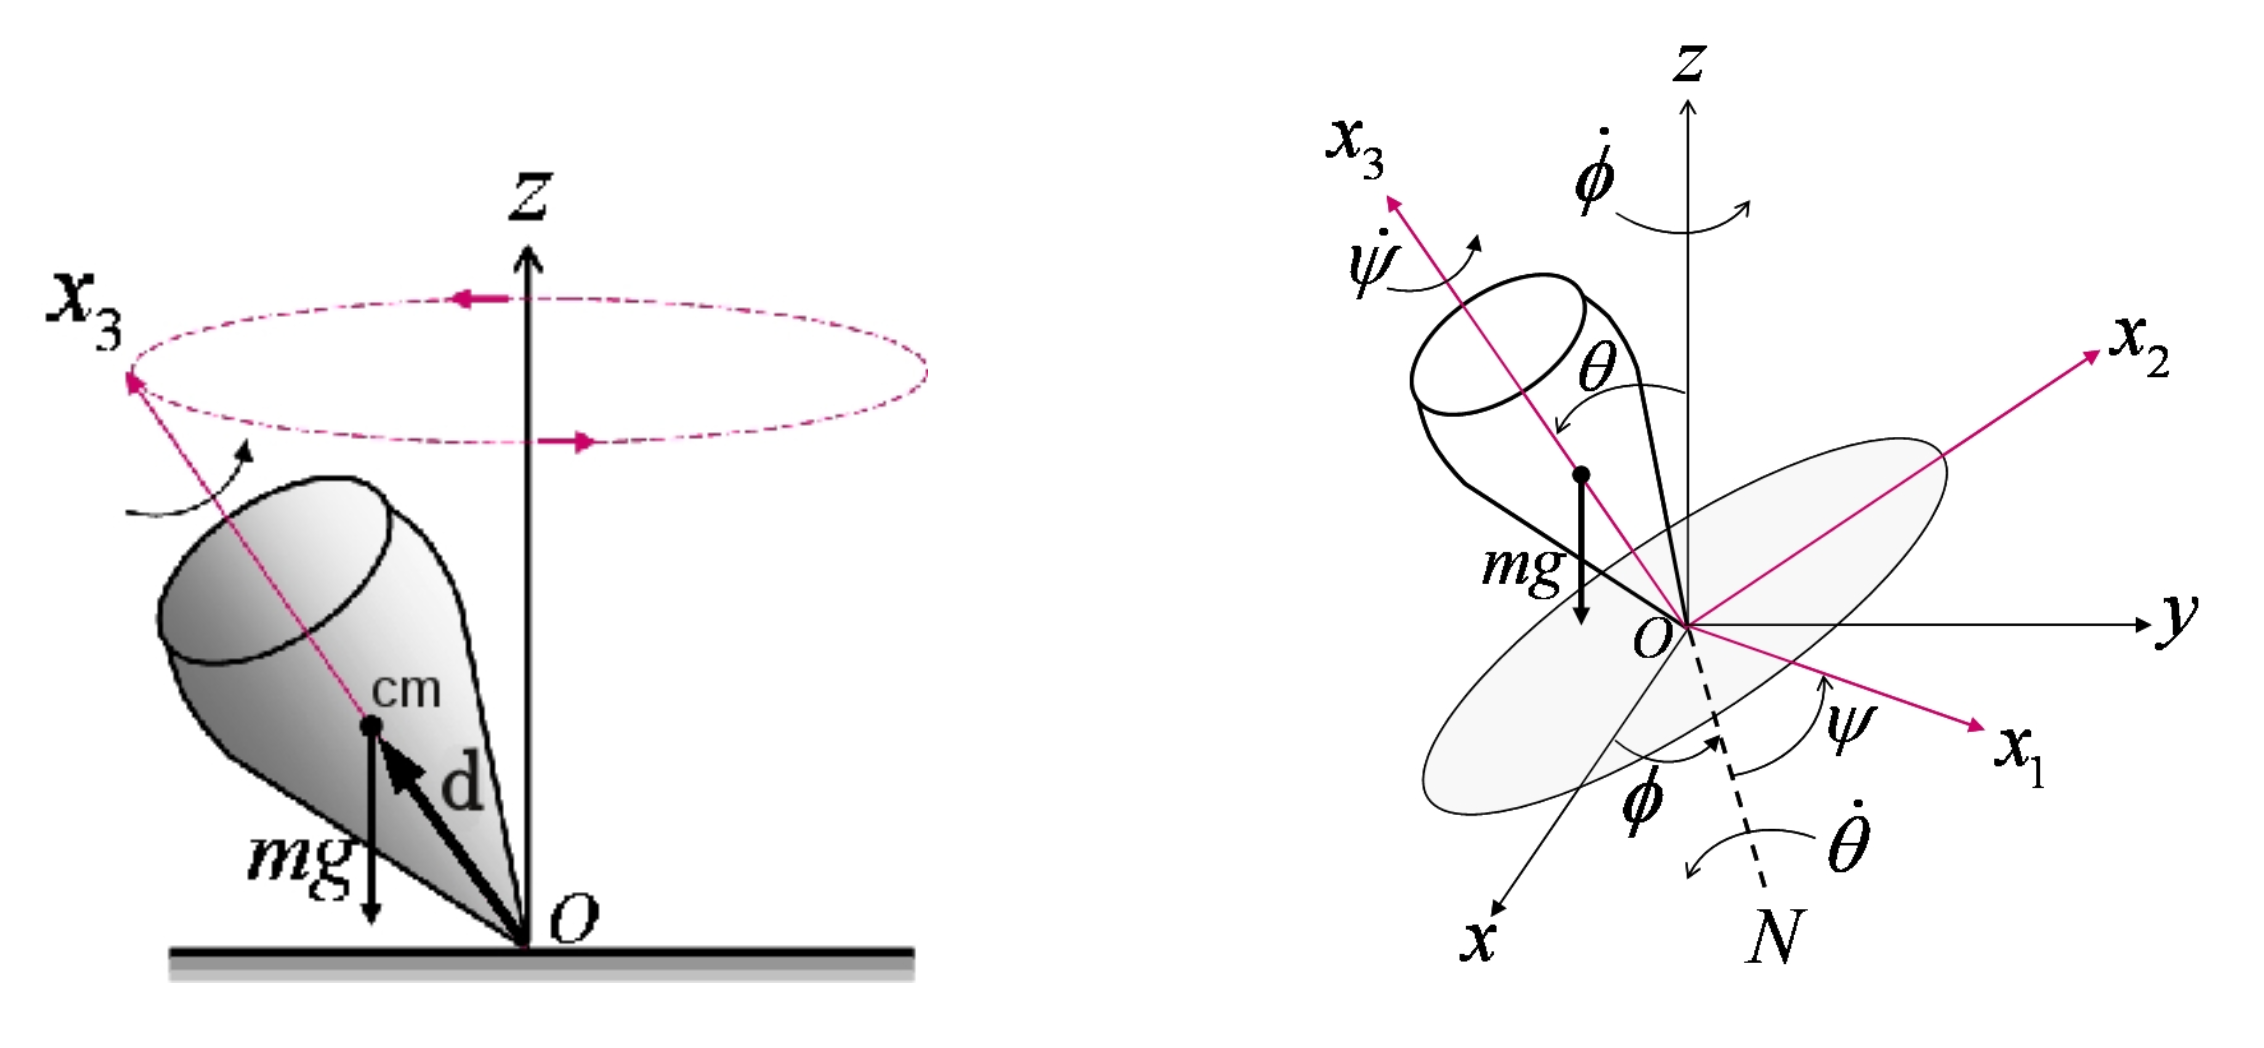
\includegraphics[width=2.1in]{Figuras/TrompoLagrange.png}
   	\end{figure}
	\item<3-> Los momentos de inercia $I_{11}^{\mathrm{cm}}=I_{22}^{\mathrm{cm}} \neq I_{33}^{\mathrm{cm}}$ son los momentos de inercia del trompo con respecto a su centro de masa.
	\item<4-> Tomamos el sistema del laboratorio $(x, y, z)$ y el sistema $\left(x_1, x_2, x_3\right)$ fijo en el cuerpo, ambos con origen en $O$.
	\item<5-> Sea $\mathbf{d}=(0,0, d)$ la posici�n del centro de masa del trompo con respecto a $O$ en el sistema $\left(x_1, x_2, x_3\right)$.
    \end{itemize}
}
%%%%% Diapo 2
\section{El Trompo de Lagrange: El Lagrangeano}
\frame{
\frametitle{El Trompo de Lagrange: El Lagrangeano}
\begin{itemize}  
	\item<1-> Consideremos los momentos de inercia respecto al sistema $\left(x_1, x_2, x_3\right)$ fijo en el cuerpo con origen en $O$, ubicado en $\mathbf{a}=-\mathbf{d}$ con respecto al centro de masa.
	\item<2-> Los momentos de inercia con respecto a los ejes $\left(x_1, x_2, x_3\right)$ del sistema centrado en $O$ son $I_{i k}=I_{i k}^{\mathrm{cm}}+m\left(a^2 \delta_{i k}-a_i a_k\right)$.
	\item<3-> Por lo tanto $I_{11} =I_{11}^{\mathrm{cm}}+m d^2$, $I_{22}  =I_{22}^{\mathrm{cm}}+m d^2$  y $I_{33} =I_{33}^{\mathrm{cm}} \neq I_{11}=I_{22}$
	\item<4-> La energ�a potencial del trompo, con respecto a $O$, es $V=m g z=m g d \cos \theta$.
	\item<5-> La energ�a cin�tica del trompo se debe a la rotaci�n con respecto al punto fijo $O$, $T_{\mathrm{rot}}=\frac{1}{2}\left(I_{11} \Omega_1^2+I_{22} \Omega_2^2+I_{33} \Omega_3^2\right)$
	\item<6-> Las componentes de la velocidad angular $\boldsymbol{\Omega}$ se pueden expresar en funci�n de los �ngulos de Euler como $T_{\text {rot }}=\frac{1}{2} I_{11}\left(\dot{\theta}^2+\dot{\phi}^2 \operatorname{sen} ^2 \theta\right)+\frac{1}{2} I_{33}(\dot{\psi}+\dot{\phi} \cos \theta)^2$
	\item<7-> El Lagrangiano del sistema es $\mathcal{L} =T_{rot} -V=\frac{1}{2} I_{11}\left(\dot{\theta}^2+\dot{\phi}^2 \operatorname{sen} ^2 \theta\right)+\frac{1}{2} I_{33}(\dot{\psi}+\dot{\phi} \cos \theta)^2-m g d \cos \theta$.
\end{itemize}
}
%%%%% Diapo 2
\section{El Trompo de Lagrange: Coordenadas c�clicas y cantidades conservadas}
\frame{
\frametitle{Coordenadas c�clicas y cantidades conservadas}
\begin{itemize}  
	\item<1-> El sistema posee tres grados de libertad: los �ngulos de Euler $\theta, \phi$ y $\psi$
	\item<1-> No depende del tiempo y tiene dos coordenadas c�clicas: $\psi$ y $\phi$.
	\item<2-> La ecuaci�n de Lagrange para $\psi$ (c�clica) es $\frac{d}{d t}\left(\frac{\partial \mathcal{L}}{\partial \dot{\psi}}\right)-\frac{\partial \mathcal{L}}{\partial \psi}=0$
	\item<2-> Entonces, $\frac{\partial \mathcal{L}}{\partial \psi}  =0 \Rightarrow \frac{\partial \mathcal{L}}{\partial \dot{\psi}}  =I_{33}(\dot{\psi}+\dot{\phi} \cos \theta)=I_{33} \Omega_3=l_3=$ cte. 
	\item<3-> La ecuaci�n de Lagrange para $\phi$ (c�clica) es $\frac{d}{d t}\left(\frac{\partial \mathcal{L}}{\partial \dot{\phi}}\right)-\frac{\partial \mathcal{L}}{\partial \phi}=0$
	\item<3-> Otra vez \\ $\frac{\partial \mathcal{L}}{\partial \phi}  =0 \Rightarrow \frac{\partial \mathcal{L}}{\partial \dot{\phi}}  =\left(I_{11} \operatorname{sen} ^2 \theta+I_{33} \cos ^2 \theta\right) \dot{\phi}+I_{33} \dot{\psi} \cos \theta=L_z=$ cte.
	\item<4-> El torque externo del peso $\boldsymbol{\tau}=-m g \hat{\mathbf{z}} \times \mathbf{d}=m g d\left(\hat{\mathbf{z}} \times \hat{\mathbf{x}}_3\right)$, es perpendicular al plano $\left(x_3, z\right)$, al igual que el vector $d \mathbf{L}$ del cambio de momento angular del trompo.
	\item<5-> No hay componentes del torque en las direcciones $\hat{\mathbf{x}}_3$ ni  $\hat{\mathbf{z}}$, es decir no hay  cambios del vector momento angular en esas direcciones, por lo que $L_3=$ cte y $L_z=$ cte.
	\item<6-> La energ�a se conserva $E=\frac{1}{2} I_{11}\left(\dot{\theta}^2+\dot{\phi}^2 \operatorname{sen} ^2 \theta\right)+\frac{1}{2} I_{33}(\dot{\psi}+\dot{\phi} \cos \theta)^2+m g d \cos \theta=$ cte. 
\end{itemize}
}
%%%%% Diapo 2
\section{El Trompo de Lagrange: Primeras integrales}
\frame{
\frametitle{Primeras integrales}
\begin{itemize}  
	\item<1-> El trompo de Lagrange es un sistema integrable: posee tres grados de libertad ( $\psi, \phi$ y $\theta$ ) y tres cantidades conservadas $\left(L_3, L_z\right.$ y $E$ ).
	\item<2-> Las primeras integrales del sistema ser�n: \\ $\dot{\phi}  =\frac{\left(L_z-L_3 \cos \theta\right)}{I_{11} \operatorname{sen} ^2 \theta}$ \\
	$\dot{\psi} =\frac{L_3 - I_{33} \dot{\phi} \cos \theta }{I_{33}} = \frac{L_3}{I_{33}}-\frac{(L_z-L_3 \cos \theta ) \cos \theta}{I_{11} \operatorname{sen}^2 \theta}$ \\
	$\dot{\theta}= \sqrt{\frac{2}{I_{11}}\left(E -\frac{\left(L_z-L_3 \cos \theta\right)^2}{2 I_{11} \operatorname{sen} ^2 \theta}-\frac{L_3^2}{2 I_{33}}+m g d \cos \theta \right)}$
	\item<3-> Podemos reescribir
	$E^{\prime}  =E-\frac{L_3^2}{2 I_{33}}=\frac{1}{2} I_{11} \dot{\theta}^2+V_{\mathrm{ef}}(\theta)=$cte, con 
	$V_{\mathrm{ef}}(\theta) =\frac{\left(L_z-L_3 \cos \theta\right)^2}{2 I_{11} \operatorname{sen} ^2 \theta}+m g d \cos \theta$
	\item<4-> Es un problema unidimensional para la coordenada $\theta$, con un potencial efectivo $V_{\text {ef }}(\theta)$
\end{itemize}
}
%%%%% Diapo 2
\section{El Trompo de Lagrange: Potencial efectivo}
\frame{
\frametitle{El Trompo de Lagrange: Potencial efectivo}
\begin{itemize}  
	\item<1-> El potencial efectivo $V_{\text {ef }}(\theta)$ tiene un m�nimo para $\theta_0$ en $\left.\frac{\partial V_{\mathrm{ef}}}{\partial \theta}\right|_{\theta_0}=0$
	\begin{figure}[t]
		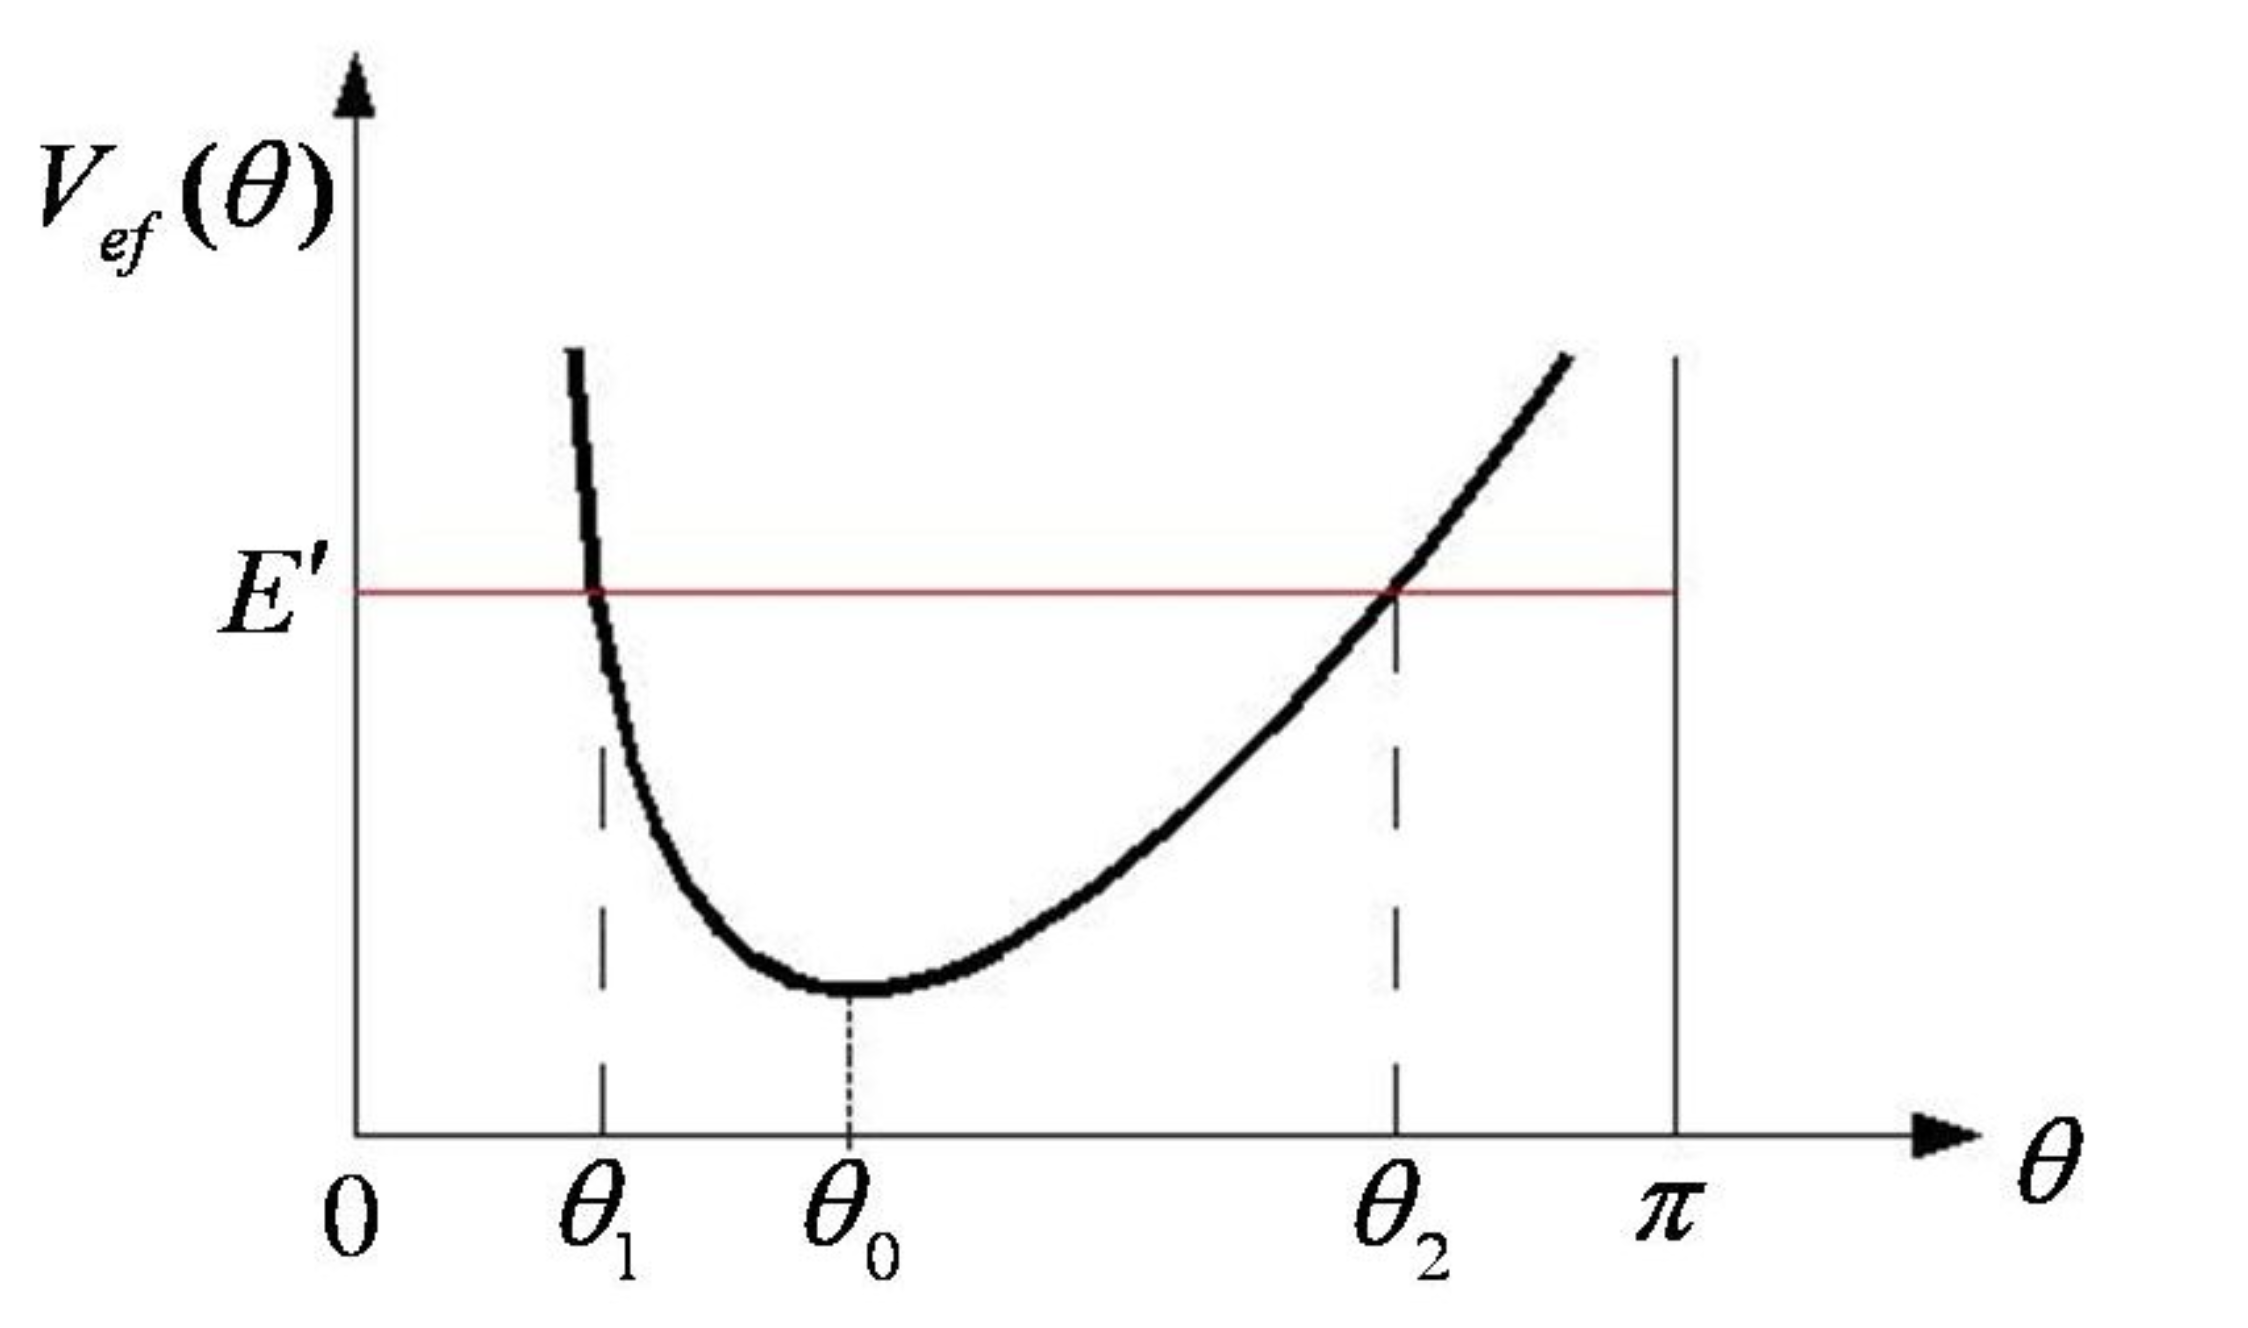
\includegraphics[width=1.8in]{Figuras/MinPotencialTrompo.png}
   	\end{figure}
	\item<2-> Los �ngulo $\theta$ posibles ocurren para valores $E^{\prime} \geq V_{\text {ef }}(\theta)$
	\item<3-> Los puntos de retorno $\theta_1$ y $\theta_2$ son soluciones de la ecuaci�n $E^{\prime}=V_{\mathrm{ef}}(\theta)=\frac{\left(L_z-L_3 \cos \theta\right)^2}{2 I_{11} \operatorname{sen} ^2 \theta}+m g d \cos \theta$
	\item<4-> La nutaci�n ocurre en el intervalo $\theta \in\left[\theta_1, \theta_2\right]$
	\item<5-> De la energ�a obtuvimos 
	$\dot{\theta}=\frac{d \theta}{d t}=\sqrt{\frac{2\left(E^{\prime}-V_{\mathrm{ef}}(\theta)\right)}{I_{11}}}, \Rightarrow 
 t(\theta)=\sqrt{\frac{I_{11}}{2}} \int \frac{d \theta}{\sqrt{\left(E^{\prime}-V_{\mathrm{ef}}(\theta)\right)}} $

\end{itemize}
}
%%%%% Diapo 2
\section{El Trompo de Lagrange: Nutaci�n y rotaci�n}
\frame{
\frametitle{El Trompo de Lagrange: Nutaci�n y rotaci�n}
\begin{itemize}  
	\item<1-> El per�odo de nutaci�n es $T_{\mathrm{nut}}=2 \sqrt{\frac{I_{11}}{2}} \int_{\theta_1}^{\theta_2} \frac{d \theta}{\sqrt{\left(E^{\prime}-V_{\mathrm{ef}}(\theta)\right)}}$
	\item<2-> La velocidad angular de precesi�n $\dot{\phi}$, puede cambiar su direcci�n instant�nea en los puntos de retorno $\theta_1$ y $\theta_2$, dependiendo del signo de $\left(L_z - L_3 \cos \theta\right)$
	\item<3-> Cuando $\dot{\phi}>0$ siempre $\left(L_z>L_3 \cos \theta, \forall \theta\right)$.
	\item<4-> Cuando $\dot{\phi}$ cambia de signo en $\theta_1$ � en $\theta_2$, dependiendo del signo de la cantidad ( $L_z-L_3 \cos \theta_{1,2}$ ) (el sentido del movimiento depende de condiciones iniciales).
	\item<5-> Cuando $\dot{\phi}=0$ en $\theta_1$ � en $\theta_2\left(L_z=L_3 \cos \theta_{1,2}\right)$.
	\begin{figure}[t]
		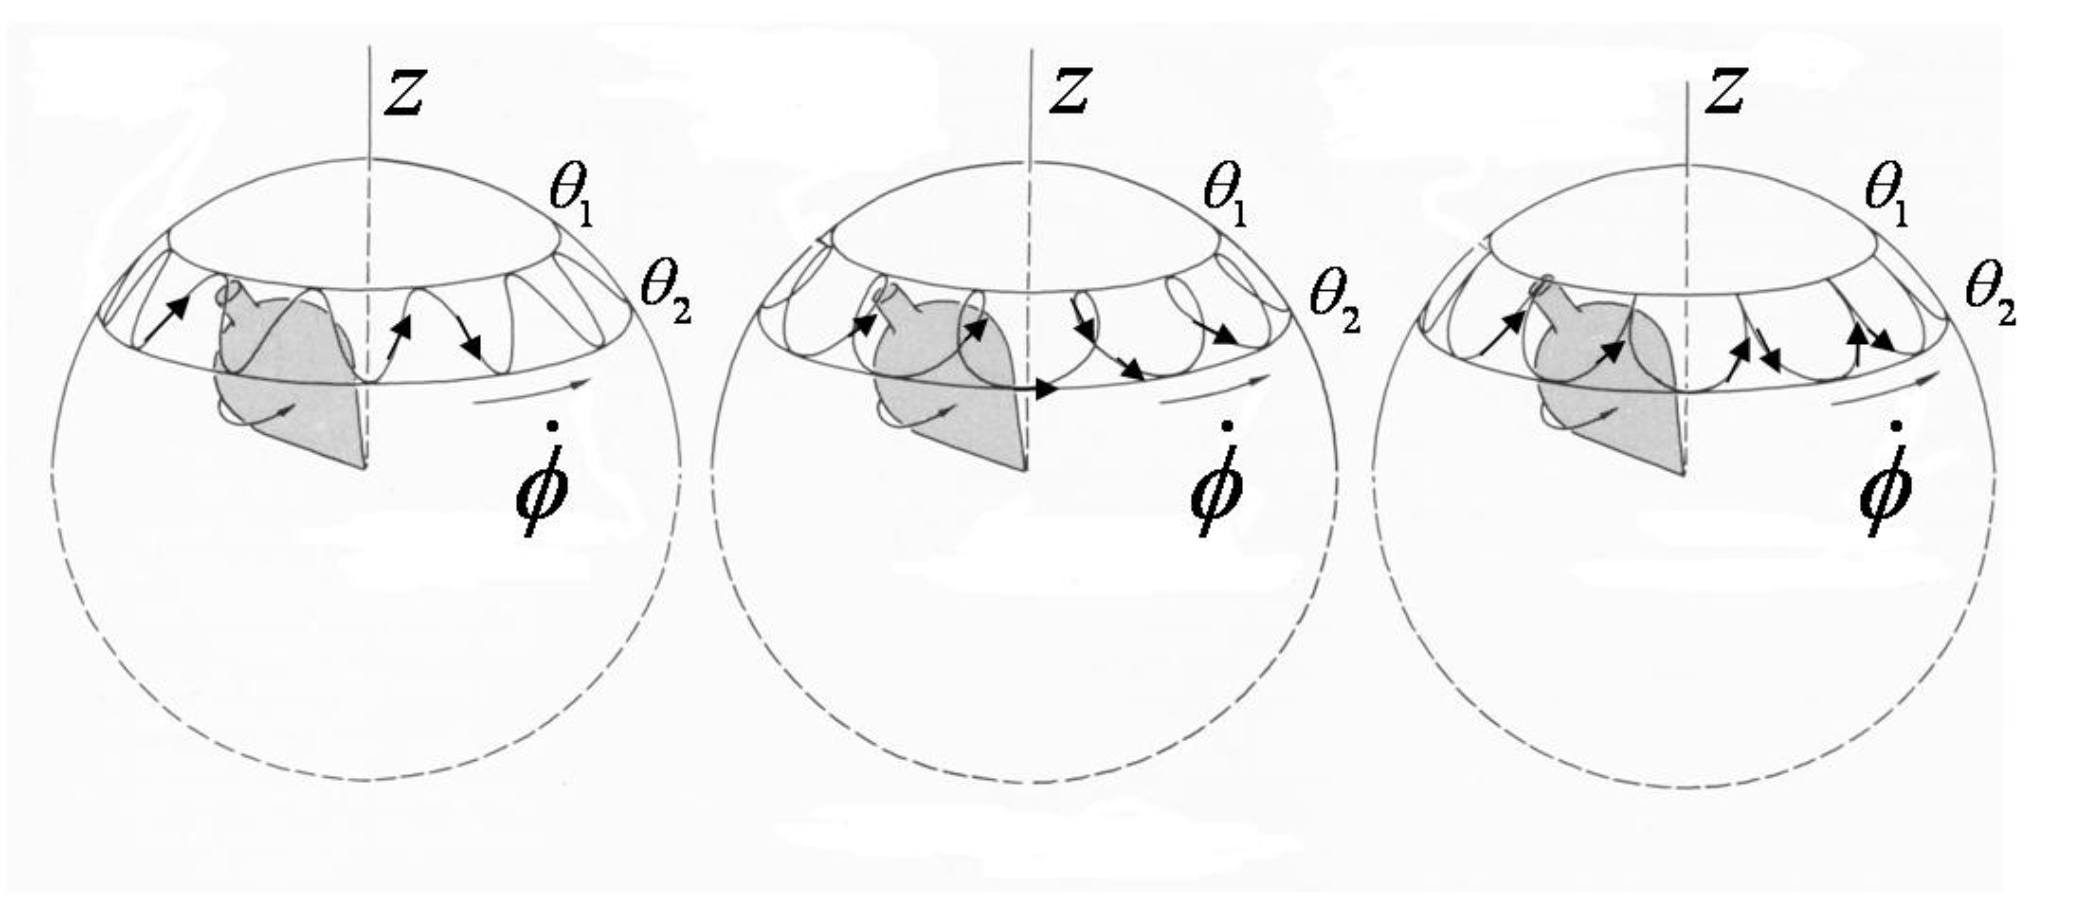
\includegraphics[width=2.2in]{Figuras/NutacionTrompo.png}
   	\end{figure}
\end{itemize}
}
  
\end{document}
%%%%% Diapo 2
\section{Secci�n}
\frame{
\frametitle{T�tulo transparencia}
\begin{itemize}  
	\item<1-> 
\end{itemize}
}

	\begin{figure}[t]
		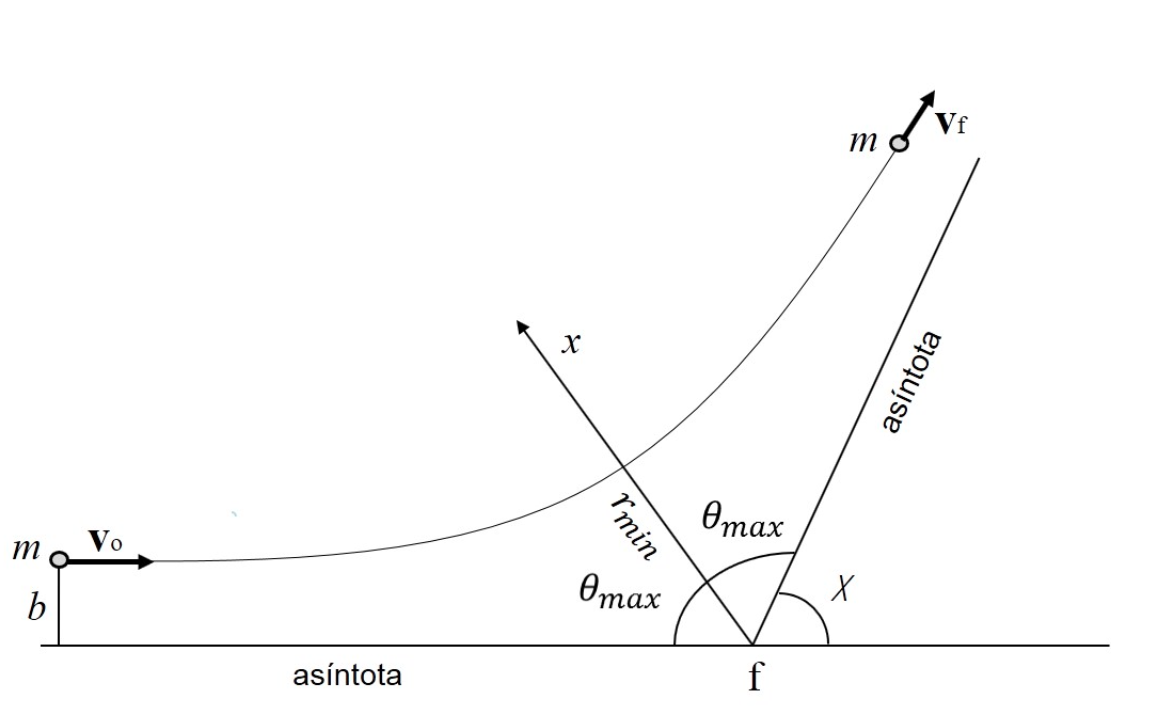
\includegraphics[width=1.8in]{Figuras/Dispersion.png}
   	\end{figure}
	
